\documentclass{beamer}

% packages
\usepackage{graphicx}
\usepackage{enumitem}

% metadata
\title{ECE 453 Project Proposal}
\author{Vaughn Kottler}
\author{Mayank Katwal}
\author{Cooper Green}
\date{\today}

\begin{document}

% title slide
\begin{frame}
\begin{center}
{\Large\textbf{Fault-Tolerant Quadcopter}}\\
\vspace{\baselineskip}
ECE 453 Project Proposal (Fall 2018)\\
University of Wisconsin-Madison\\
\vspace{\baselineskip}
{\large\textit{Vaughn Kottler, Mayank Katwal, Cooper Green}}
\end{center}
\end{frame}

% top-level block diagram
\begin{frame}
\frametitle{Overview}
\begin{center}
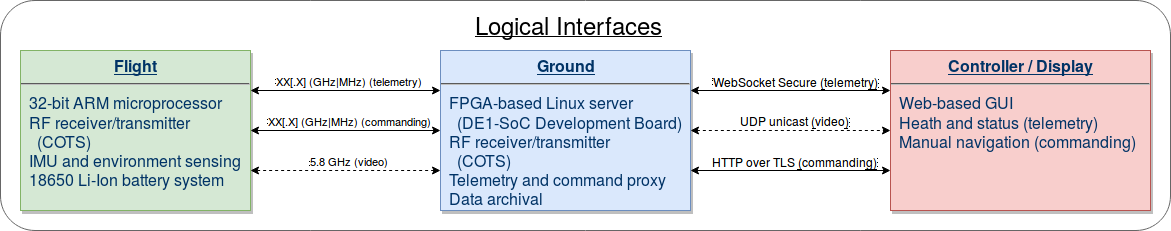
\includegraphics[width=\linewidth]{../src/im/top_level}
\end{center}
\vspace{\baselineskip}
\begin{description}[align=right,labelwidth=80pt,itemsep=10pt]
\item [Quadcopter] -- Battery-powered, four-motor flying machine
\item [Ground Station] -- Linux server managing the quadcopter's
	radio endpoint, hosts wired-network services (i.e.\ telemetry)
\item [Web-based UI] -- A modern dashboard for visualizing data
	and manually commanding the vehicle
\end{description}
\end{frame}

% learning objectives
\begin{frame}

\frametitle{Learning Objectives}

Exposure to:
\begin{itemize}[itemsep=10pt]
	\item [--] Radio-frequency communication
	\item [--] Control theory
	\item [--] System-level engineering
	\item [--] SoC platform(s)
\end{itemize}

\vspace{\baselineskip}

Also:
\begin{itemize}[itemsep=10pt]
	\item [--] Data pipelining in the aerospace/avionics problem space
	\item [--] Modern user-interface design and implementation
\end{itemize}

\end{frame}

% features
\begin{frame}
\frametitle{Features}
\begin{description}[align=right,labelwidth=100pt,itemsep=10pt]
	\item [Single-Fault Tolerant] -- Land safely in the event of communication
		``heartbeat timeout''
	\item [Telemetry Archival] -- Implement long-term telemetry storage for
		post-flight data analysis
\end{description}
\end{frame}

% quadcopter
\begin{frame}
\frametitle{Quadcopter}
\begin{center}
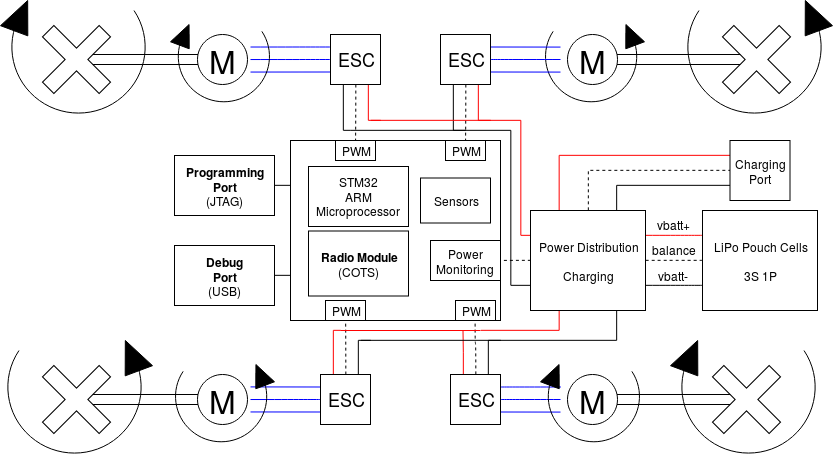
\includegraphics[width=\linewidth]{../src/im/quadcopter}
\end{center}
\end{frame}

% ground station
\begin{frame}
\frametitle{Ground Station}
\begin{center}
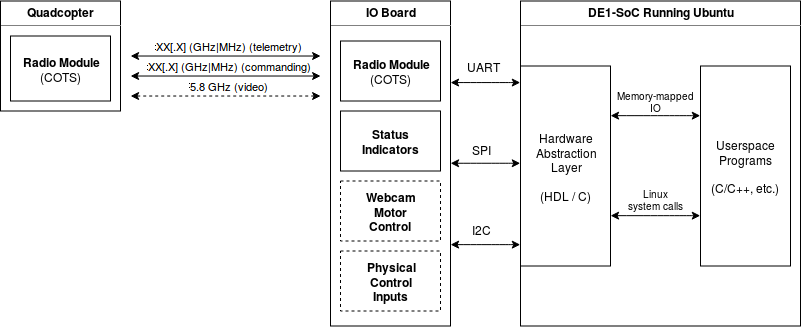
\includegraphics[width=\linewidth]{../src/im/ground_station}
\end{center}
\end{frame}

% display and controller
\begin{frame}
\frametitle{User Interface}
\begin{center}
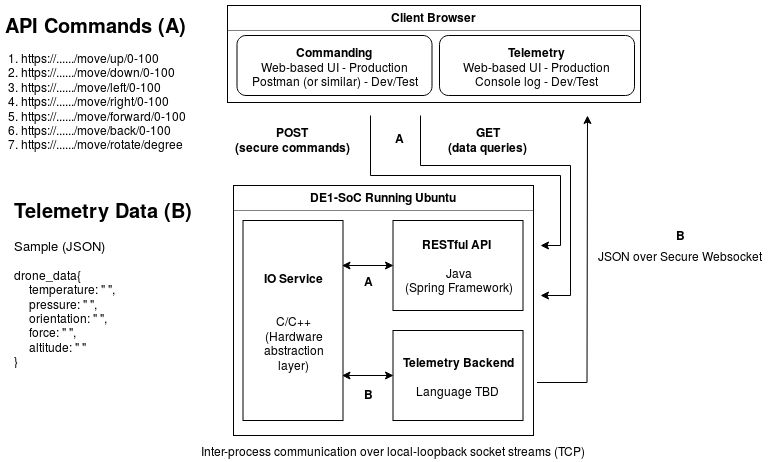
\includegraphics[height=225pt,width=\linewidth,keepaspectratio]{../src/im/display_controller}
\end{center}
\end{frame}

% milestones 1
\begin{frame}
\frametitle{Milestones}
\begin{enumerate}[label=\arabic*),itemsep=10pt]
	\item Establish wireless communication between the vehicle and
		ground station
	\item Establish percentage-based throttle control over each motor
	\item Establish manual-commanding capability to the vehicle from a
		web-based user interface
	\item View live telemetry from a web-based user interface
	\item Sense angular velocity via gyroscope and force experienced via
		inertial measurement unit
\end{enumerate}
\end{frame}

% milestones 2
\begin{frame}
\frametitle{Milestones cont.}
\begin{enumerate}[start=6,label=\arabic*),itemsep=10pt]
	\item Develop a control algorithm to fly in a stable hover or
		holding pattern
	\item Extend control algorithm to control for velocity in three axes
		to achieve controlled motion
	\item Sense relative altitude
	\item Extend control algorithm to control for a specific \textit{delta-y}
		(perpendicular to ground plane) 
\end{enumerate}
\end{frame}

% workflow 1
\begin{frame}
\frametitle{Initial Development and Prototyping}
\begin{center}
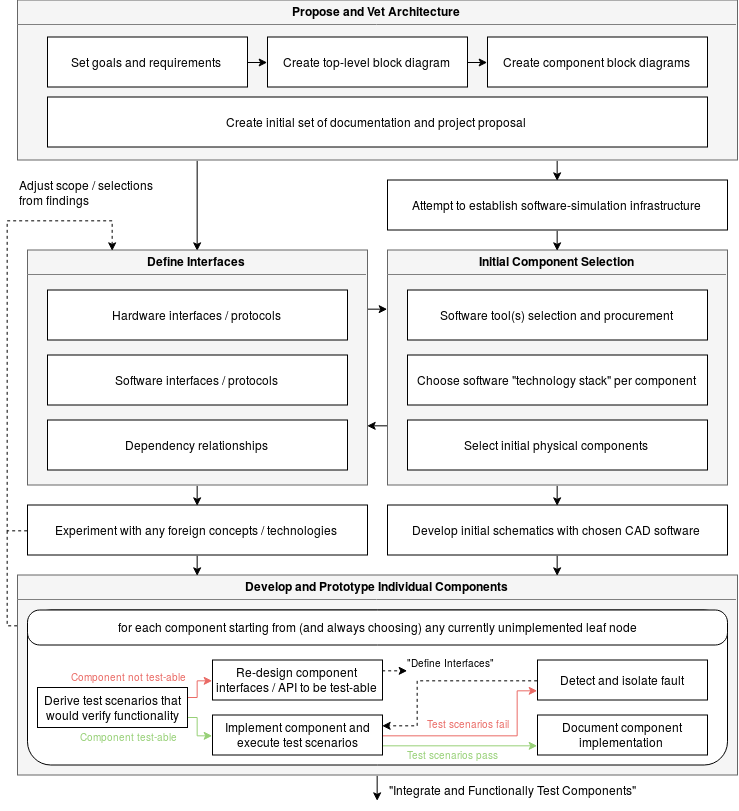
\includegraphics[height=200pt,width=\linewidth,keepaspectratio]{../src/im/workflow_1}
\end{center}
\end{frame}

% workflow 2
\begin{frame}
\frametitle{Final Stages}
\begin{center}
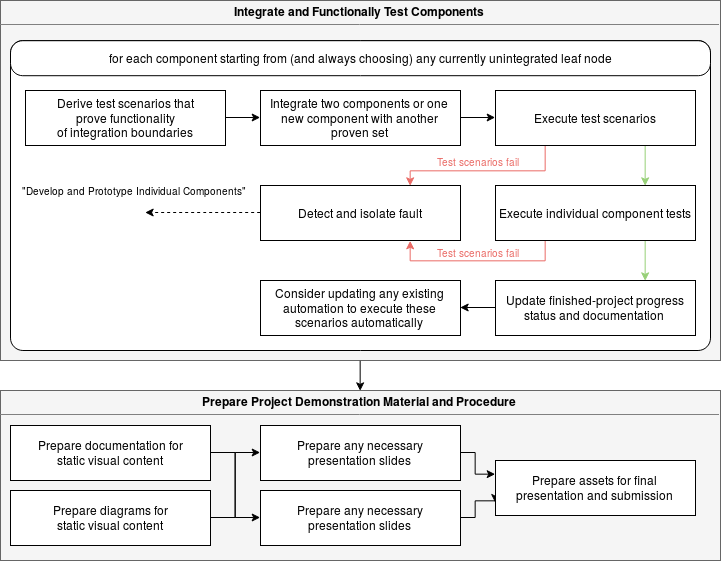
\includegraphics[height=200pt,width=\linewidth,keepaspectratio]{../src/im/workflow_2}
\end{center}
\end{frame}

\end{document}
